% Created 2020-06-01 Mon 19:59
% Intended LaTeX compiler: pdflatex
\documentclass[11pt]{article}
\usepackage[utf8]{inputenc}
\usepackage[T1]{fontenc}
\usepackage{graphicx}
\usepackage{grffile}
\usepackage{longtable}
\usepackage{wrapfig}
\usepackage{rotating}
\usepackage[normalem]{ulem}
\usepackage{amsmath}
\usepackage{textcomp}
\usepackage{amssymb}
\usepackage{capt-of}
\usepackage{hyperref}
\usepackage{todonotes}
\author{Njagi Mwaniki and you if you wanna ;)}
\date{}
\title{A Review of Genome Graph Tools}
\hypersetup{
 pdfauthor={Njagi Mwaniki and you if you wanna ;)},
 pdftitle={A Review of Genome Graph Tools},
 pdfkeywords={},
 pdfsubject={},
 pdfcreator={Emacs 26.3 (Org mode 9.2.4)}, 
 pdflang={English}}
\begin{document}

\maketitle

\section{Abstract}
\label{sec:org9e67f3a}
\todo{add abstract}

\section{Introduction}
\label{sec:orgcf5dca6}

There are four major overlapping steps that need to be carried out after DNA sequencing to get actionable results. 
fragment assembly which involves recreating the original genetic sequence;
alignment, mapping, indexing and querying which are part of the 
assembly stage but can be done later to query the relatedness of sequences;
and Visualization: to see these changes.
\todo{expand this intro}

\section{Fragment Assembly}
\label{sec:org0051fa5}
The fragment assembly problem is solved in 4 main stages 1) Assemble a graph, 2)
Simplify the graph, 3) Map reads to the graph, and 4)Produce the assembly.

By defining the assembly problem this way it becomes a problem of finding a set
of common super-strings from a set of substrings.
Tools take either a Eulerian, connect the nodes, or a Hamiltonian, connect the 
edges, approach to this problem.

Sanger sequencing brought about the fragment assembly problem. 
Solutions to the fragment assembly problem started with SEQAID 
(Peltola et al 1984) whose solution was the Overlap Layout Consensus (OLC) 
framework, an intuitionistic approach to the assembly problem that works in 
3 main steps: 1) Overlap: find all overlaps among the reads, 2) Layout: assemble 
a graph of all the reads based on their overlaps, and 3) Consensus: infer the 
consensus sequence.

“In the first phase, 5′ and 3′ poor regions of each read are identified and removed. 
Overlaps between reads are computed. False overlaps are identified and removed. 
In the second phase, reads are joined to form contigs in decreasing order of overlap scores.
 Then, forward–reverse constraints are used to make corrections to contigs. 
In the third phase, a multiple sequence alignment of reads is constructed and a
 consensus sequence along with a quality value for each base is computed for 
each contig. Base quality values are used in computation of overlaps and
 construction of multiple sequence alignments. We describe each phase in
 detail below.”

What it does is find the overlaps between the given set of reads and then lays 
them out to form a DAG. The graph, however, has multiple paths that are the 
genome or superstring in question. Which is where the consensus comes in. 
It used … to infer the consensus.

\begin{center}
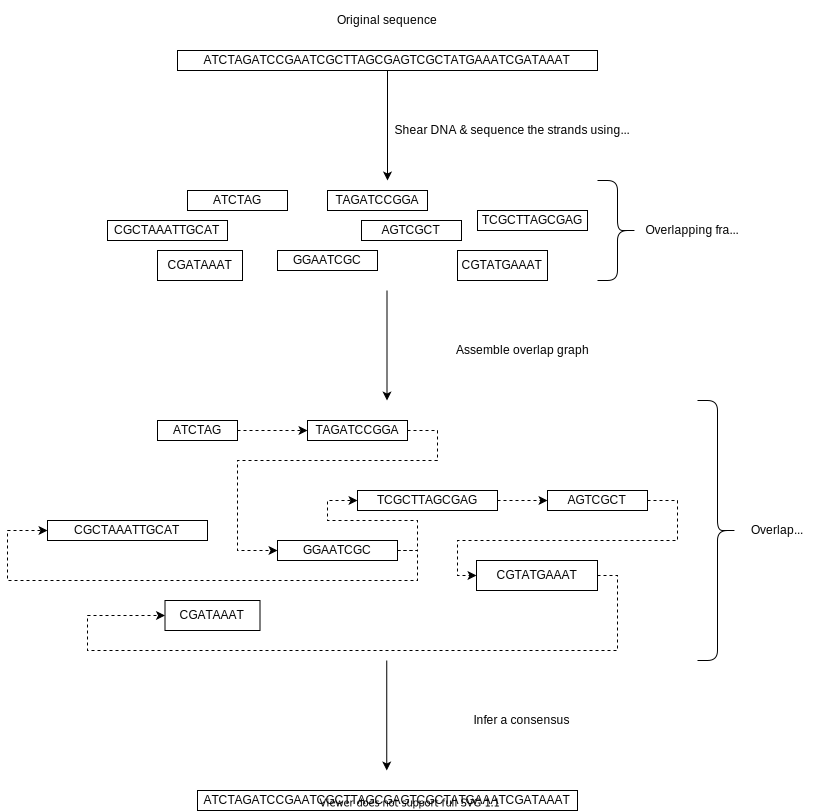
\includegraphics[width=.9\linewidth]{./assets/images/OLC framework.png}
\end{center}

With the advent of second generation sequencing (SGS) \todo{name the tech itself illumina, pyrosequencing, 454}
methods there was a significant increase in the number of reads produced which
made OLC unfeasible. 

It was progressively replaced by de Bruijn Graph (DBG) (Idury and Waterman 1995),
with the first tool was EULER (Pevzner, Tang and Waterman 2001), 
based methods which made it possible to work with the increasing number of reads
produced. 
DBG uses an anti-intuitionistic solution whose assembly quality improves with an 
increase in the read length <cn>.
 It works through: chop the reads into much smaller k-mers, Use all the kmers 
to assemble a dBG, Infer the genome sequence on the dBG.

\begin{center}
\includegraphics[width=.9\linewidth]{./assets/images/de Bruijn Graph.png}
\end{center}

“In OLC assembly using the reads graph, the layout step is a Hamiltonian path 
problem, which is known to be NP-hard; however, in DBG assembly using the k-mer 
graph, inferring the contig sequence is an Euler path problem that is easier to 
resolve (\url{https://doi.org/10.1073/pnas.171285098}). Therefore, the main advantage 
of DBG is that it transforms assembly problems to an easier problem in algorithm 
theory.”

Lately, Single Molecule Sequencing (long read sequencing)  methods have 
reintroduced OLC for the assembly of long erroneous reads but DBG based methods 
are still used to correct long reads.
The unitig approach involves finding the maximal interval subgraphs in the
graph of all read overlaps.
The string graph (Myers,. 2005)  is a way to infer the genome from the read data
without a need for k-mers as is with the de Bruijn graph.  
It treats the genome as a sequence of repeats and then “encodes” each repeat as 
a node. Each unique (contiguous) sequence is a node. 
An Eulerian tour recreates the genome.

\begin{center}
\includegraphics[width=.9\linewidth]{./assets/images/String Graph.png}
\end{center}

\section{Alignment and mapping}
\label{sec:org6ca859e}
Sequence alignment started with the (Needleman and Wunsch 1970) solution to the edit distance problem. Theirs was a dynamic programming approach which had a complexity of O(n2); this was then known as global alignment. It was followed by semi-global alignment (Sellers, 1980) where one sequence (query) is entirely aligned to a substring of the other (reference) then local alignment (Smith and Waterman, 1981), where the alignment can be between any substrings of the two sequences.
Alignment involves finding the closest match between two strings. This can involve trying to find the shortest edit distance between two strings (global alignment) or finding where a substring lies within a larger string either exactly or approximately (fuzzy) within a larger one (local and semi-global alignment).
Before alignment a complement of each read is generated to be searched against because of the direction of sequencing or inversions. A match can either be exact, matching the pattern exactly, or fuzzy, where a section or all of the string matches the pattern approximately, with minimum edit distance.
Alignment problems grow with the input size (citePBWT paper?). This makes it hard to align to graphs because of the sheer amount of data involved where the complexity of an alignment problem is a function of the number of  vertices |V| and edges |E| <cn>.  In this case a read is mapped to a  path in the graph instead of linear sequences. In some way you can think of it as mapping to multiple linear sequences that may or may not loop.

\section{Indexing}
\label{sec:orga42fb9c}
The indexing and alignment problem are two sides of the same coin. We need an indexing scheme to speed up alignment and make it pragmatic within the given time and memory requirements. Indexing is therefore an “economic” solution to the problem of search given limited computing resources. It involves reducing the search space so as to reduce the time taken and memory consumed when performing a search.
In linear references commonly used indexing approaches are the FM index <list tools> whose complexity is O(NM) where there are N variable sites and M sequences (Durbin 2014).
As in alignment the problem grows even larger with the proliferation of paths in graphs. For graphs, indices like the FM-index backed by the BWT fail to hold and there’s the need for improvements such as that seen in gBWT used in seqwish allowing it to be orders of magnitude faster than VG.
An index can either be static or dynamic. A static index is serialized and saved to disk while a dynamic index is created at runtime and held in memory. Dynamic indices are good with small datasets that change rapidly such as in the construction of a DBG making it suitable for fragment assembly. Static indices are suited for larger datasets that we want to go back to such as a reference genome graph.

\section{Approaches}
\label{sec:org7751a48}
\subsection{BWT}
\label{sec:orgbb9fc2e}
Introduced by (Burrows and Wheeler, 1994) for string data compression, forms the basis of the bzip compression algorithm.
Can be compressed with run length encoding where like bases end up clustering together in runs enabling them to be stored in a more terse form.

\begin{center}
\includegraphics[width=.9\linewidth]{./assets/images/Run Length Encoding.png}
\end{center}

\subsection{Suffix Array}
\label{sec:org5f07f45}
Suffix arrays invented by (Manber and Myers 1990) are arrays of the positions of all the sorted suffixes of a string. Its aim is to be a simple, space efficient (stores n integers where n is the length of the string) alternative to the suffix tree <citation needed> whose space requirements are\ldots{}
based on BWT have been used for fast search algorithms
Improvement to the suffix array: (Li, Li \& Huo 2016) gave the first in-place  O(n) time suffix array construction algorithm that is optimal both in time and space, where in-place means that the algorithm only needs O(1) additional space beyond the input string and the output suffix array.
Tools using the suffix array
Bowtie (Langmead et al., 2009)
BWA (Li and Durbin, 2009)
SOAP2 (Li et al., 2009)

\subsection{FM Index}
\label{sec:org293f541}
Short for Full-text index in Minute space; the FM-index created by (Ferragina and Manzini, 2000) is a full text substring index based on the BWT. It allows compression of the input text while permitting fast substring queries.
It can be used to efficiently find the number of occurrences of a pattern within the compressed text, as well as locate the position of each occurrence.

\subsection{PBWT}
\label{sec:orgd9e057a}
Introduced by  (Durbin 2014) Positional Burrows Wheeler Transform is an algorithm with complexity O(NM) where M sequences and N bi-allelic sites.
It derives a representation of the data based on a positional prefix array; an array that holds positions of a given array/set of haplotypes in a larger haplotype array. This prefix array orders them in reverse (ascending) order of their prefixes allowing similar sequences to cluster together.

<Add PBWT table and graphic>

\subsection{GBWT/gPBWT}
\label{sec:orga3967c7}
First described (Novak et al,. 2016) but used in a tool (Siren et al., 2020) it’s a compressible representation of a set of haplotypes held in the graph. This allows for efficient match queries in sections of the haplotypes (local alignment). Because of the previously mentioned nature of the positional suffix array to bring together (fairly) similar haplotypes. GBWT lets us have an efficient way of counting the number of haplotypes containing a given sequence.

\subsection{Bloom filters}
\label{sec:org4215751}
The bloom filter is a probabilistic data structure that can give false positive but never a false negative.  It works by hashing data and stores the hash in an array\ldots{}
It is suited for the fragment assembly using DBGs because of its constant time access (Chikhi et al, 2013). It however suffers from poor data localization <expound> which led to the use of Blocked Bloom Filters (BBF) (Putze et al,. 2010) used in Bifrost (Holley \& Melsted, 2019).

\subsection{Minimizers}
\label{sec:orgd9868a7}
The work of a minimizer is to reduce the search space. It does this by generating kmers from a read and sorting them alphabetically. The k-mer at the top is the minimizer for that read\ldots{} then binning the result. When a query is made it’s prefix is checked against the bin and the rest of the data ignored <is this even accurate?>
We can get a minimizer by BBF blocked bloom filter Minimizers (Grabowski et al., 2015; Roberts et al., 2004)

\subsection{Hash tables}
\label{sec:orgcdfe9d2}
Hash tables involve breaking down the reads into k-mers and storing the kmers into hash tables that point to the original data. When queries are made they’re similarly broken down into k-mers of the expected size<citation needed>. Hash based methods when well tuned can be faster than suffix array based methods, because the basic operations are simpler, but they typically require greater memory, particularly in cases where the suffix representation can be compressed as it can be here (Durbin 2014).
Many times tools take a hybrid approach; incorporating different aspects of different indexing schemes such as in Minimap (Li,. 2020)\ldots{}
\section{Tools}
\label{sec:org93ebf4e}
The Berkeley Open Assembler (Myers 2005) uses the string graph, and borrows from the unitig algorithm. The string graph is a way to infer the genome from the read data without a need for k-mers. It treats the genome as a sequence of repeats and then “encodes” each repeat as a node. Each unique (contiguous) sequence is a node. An Eularian tour recreates the genome
Though the original DBG approach does much better than OLC it still has a high memory footprint<citation needed>.

Minia (Chikhi et al,. 2013) proposed the use (encoding) of a DBG as a bloom filter (BF) instead of storing the graph in a “traditional” set series of nodes and edges stored in <mention tool>. By design, the BF can give a false positive result but never a false negative. This brought about the probabilistic de Bruijn graph. It is obtained by inserting all the nodes of a de Bruijn graph (i.e all k-mers) in a BF. A BF has a search/access time of O(1). They then had an additional structure to remove critical false positives. It showed that the graph can be encoded with as little as 4 bits per node.
Drawbacks: 
The Bloom filter introduces false nodes and false branching.
The global structure of the graph is approximately preserved up to a certain false positive rate.
Bcalm2 (Chikhi et al,. 2016) tried to improve this by use of compacted DBG (cdBG). It allowed the problem to be doable on a PC.

\todo{<add compaction diagram>}

The use of the de Bruijn graph in fragment assembly consists of a multi-step pipeline. The most data intensive steps are usually the first three: 
nodes enumeration/k-mer counting: the set of distinct k-mers is extracted from the reads 
Compaction: all unitigs (paths with all but the first vertex having in-degree 1 and all but the last vertex having out-degree 1) are compacted into a single vertex
graph cleaning: artifacts due to sequencing errors and poly- morphism are removed from the graph

<image explaining compaction>
Minimap (Li, 2016) introduced two tools minimap, a raw read overlapper, and miniasm (Li, 2016), an assembler. Minimap uses minimizer sketches, stores k-mers in a hash table, uses sorting extensively.
SPAdes  also a toolkit does…
Variation graphs embed the paths in the graph. These paths can be used to represent haplotypes. vg, HashGraph, odgi and PackedGraph are dynamic (allow for updates to the graph while xg isn’t).

\begin{center}
\includegraphics[width=.9\linewidth]{./assets/images/Variation Graph-Page-1.png}
\end{center}

\begin{center}
\includegraphics[width=.9\linewidth]{./assets/images/Variation Graph-Page-2.png}
\end{center}

vg (Garrison et al., 2018) used the protobuf library as the graph implementation but was refactored to use the HandleGraph API as of 1.22.0. It is an end to end pangenome graph solution for de novo and incremental graph building but has large memory requirements when it comes to indexing. How it deals with cycles in the graph: unrolls the graph with cycles. The graph holds nodes in a vector. It uses hash tables to map between nodes and ids in a vector that holds the nodes. Paths are stored in a set of linked lists. A hash table maps between nodes and paths. Suffered from a problem of data duplication. Queries involve hash table lookups.
xg(Garrison, 2019) a memory-efficient succinct representation of the graph (compared to vg). It being static and having indexing of the paths using positional indices, GBWT, allows it to have fast queries making it good at  read mapping and variant calling.
Bluntification (Garg et al., 2018) removing all overlaps between nodes
seqwish (\url{https://github.com/ekg/seqwish}) transforms a set of sequences and alignments (in GFA) into its equivalent variation graph. The large memory requirements of vg are solved through the use of gBWT backed by a Generalized Compressed Suffix Array. It’s still a static index
odgi (libhandlegraph paper) Optimized Dynamic Graph Interface, uses a dynamic index and uses an in memory variation graph to perform sorting, pruning, transformation, and visualization.
HashGraph (libhandlegraph paper) has speed as its primary goal. Represents a graph as a high performance hash table. Paths are embedded as double linked lists. Edges are in vectors attached to each node they connect. Use an adjacency list which is appropriate for sparse graphs. Appropriate for small graphs <such as viruses> because it trades memory for time.
Odgi (libhandlegraph paper) is based on a node centric encoding of the graph that is designed to improve cache coherency when traversing or modifying the graph. It tries to be a pragmatic tool that achieves balance between memory usage and performance. Each nodes seq and edges are encoded in a byte array using a variable length integer,
Edges are described in terms of the relative offset of a node in a sorted graph.
PackedGraph (libhandlegraph paper) is designed to have a low memory footprint. It does this by encoding the graph mainly using linked lists.
Baum (Wang et al., 2018) By Adaptive Unique Mapping (BAUM)  improved on the OLC framework  to improve genome assembly based on SGS paired-end/mate-pair libraries.  BAUM has two modules: 
construction of the genome unique regions that are taken as the initial contigs 
iterative assembly, in which scaffolds are built, and contigs are extended and merged, aiming to reconstruct the repetitive regions along the iterations.
In this scheme, the repetitive regions are separated by the unique regions
Bifrost (Holley et al,. 2019) improved on the cdBG by adding colours and takes advantage of concurrency (parallell) to the nodes to keep track of the source of each vertex. Size of colours can grow beyond that of the nodes In the output it stores these colours in a different on a different .bfg\textsubscript{colors} file. K-mers contained in the unitigs are mapped to their colors representing the input sources (color is represented by an integer from 1 to |C| where C is the number of colors. Colors are stored in a separate array of color containers, each color container is indexed by MPHF (Minimal Perfect Hash Function) library BBHash (Limasset et al., 2017).
BF has poor data localization because one element is scattered all over which leads to CPU cache misses when inserting and querying are addressed here  (Putze et al., n.d.) for this they used (BBF) blocked bloom filter Minimizers (Grabowski et al., 2015; Roberts et al., 2004).
BBF works by building an approximation of the dBG using BBFs to filter our seq errors. BBF containing k-mers is used to build the cdBG.
GraphAlighner (Rautiainen et al,. 2019) is A tool for aligning long error prone reads to genome graphs. It performs base alignment. It uses (generalizes two linear sequence-to-sequence algorithms to graphs) two strategies: the Shift-And algorithm for exact matching (exact match of a substring to a string) and Myer’s bit-vector algorithm for semi-global alignment
Aligns sequences to graphs while exploiting bit parallelism. Makes use of Nondeterministic Finite Automaton (NFA). Store an NFA state bitvector for each node and update until no more change is necessary
Myer’s bit-vector algorithm studies the semi-global sequence-to-graph alignment problem. It seeks to find a path in a directed, node-labelled graph that has the minimum edit distance to the query sequence. Myers’ bit-vector alignment algorithm (Myers, 1999) to graphs, which proceeds along the same lines as the Shift-And algorithm, but requires some further algorithmic insights to handle nodes with an in-degree greater than one. Bitvector algo complexity grows approximately linearly with the number of vertices in the graph. The bitvector it uses is the size of the pattern we are searching for. Semi-global alignment is solved through generalizing DP edit distance problem for graphs. Semi-global alignment is used to align a shorter seq against a longer one, reference.
Shift-And algorithms (Baeza-Yates and Gonnet, 1992; Domolki, 1964, 1968) performs exact string matching to graphs. Their aim is to find a path in a directed, node-labeled graph that has a minimum edit distance (Levenshtein (1966)) to the query sequence. Shift-And algo finds exact matches between a pattern string and a text string by simulating a nondeterministic finite automaton (NFA) that matches the pattern and then feeding the text to it.
Keep shifting the bit-vector by one and bitwise AND-ing the state. Somewhat analogous to exact matching using a window of the size of the pattern.
It can handle DAGs and  graphs that may contain cycles. For DAGs, process the nodes in topological order (topological sort). For cyclic graphs no sorting.
Minigraph (Li,. 2020), for incrementally constructing reference variation graphs, is a sequence to graph mapper that incrementally constructs a pangenome graph. A graph-based data model and associated formats to represent multiple genomes while preserving the coordinate of the linear reference genome. A straightforward way to represent a pangenome store unaligned genomes in a full-text index that compresses redundancies in sequences identical between individuals (Boucher et al., 2019; Liu, Zhu, et al., 2016; Mäkinen et al., 2010) 		
The other class of methods encodes multiple genomes into a sequence graph, usually by collapsing identical or similar sequences between genomes onto a single representative sequence. The results in a pangenome graph.
GraphAlighner performs base alignment but minigraph does not. Minigraph is faster than GraphAligner and uses less memory. Minigraph is more accurate than GraphAligner. This is counter-intuitive given that GraphAligner does base alignment. Close inspection reveals that most mismapped reads by minigraph are mapped to the correct genomic loci but wrong graph paths. On the contrary, most mismapped reads by GraphAligner are mapped to wrong genomic loci. Vg didn’t work with their PacBio data. vg allows different regions in one chromosome collapsed to one segment. We call such a graph a collapsed graph. rGFA cannot encode a collapsed graph.
vg-flow (Baaijens,. 2020) attempts to reconstruct all individual haplotypes from a mixed sample at the strain level and to provide abundance estimates for the strains. It does this by\ldots{}

\section{Interfaces and APIs}
\label{sec:org0be5cfb}
The field of genome graphs is growing at an alarming rate as evidenced by the ever-growing number of tools. There is, therefore, a need to have a common way of how the tools interact with the data they operate on. One such solution is libhandlegraph.
libhandlegraph, has python bindings and is now being ported to Rust, it is a declarative approach towards graphs that defines an interface between which tools interact with the data below. The idea is to treat the graph as a larger structure to which we have pointers to called handles (similar to Unix file handles) through which we manipulate the graph. In C++ and Python, this is done using the class abstraction while in Rust the trait abstraction is used.
libhandlegraph is primarily used in vg as an abstraction layer over different backing graph implementations.
It defines a common set of attributes and operations through which we can manipulate the graph. We can then use the libhandlegraph API as a layer between an underlying graph implementation and genome graph manipulation tools we plan on building.
libbdsg (Optimized bidirected sequence graph implementations for graph genomics) is a C++ library that provides high performance implementations of sequence graphs for graph-based pangenomics applications. Tools built on top of this are PackedGraph (low memory) and HashGraph (high-performance hash tables).
vg is now using libhandlegraph through libbdsg(Eizenga et al., 2020)

\section{Plaintext graphical representations}
\label{sec:org21991be}
In the early 2000s assembly software was dominated by a few end to end assembly software (list them) <citation needed> making it hard to tweak parts of the process which led to calls (such as THE SMALL TOOLS MANIFESTO FOR BIOINFORMATICS) for small tools that perform bits of the assembly while using plaintext files as APIs.
An early attempt was FASTG, based on a directed graph (digraph), an extension to FASTA meant to represent variability in the final output of the assembly process. It encodes the sequences on arcs/edges and a vertex refers to the connection between sequences.
Like FASTA each line contains a header line which follows the pattern >Edge:Neighbours:Properties; Where Edge is the name given to this edge/sequence, Neighbors is a list of edges (or their reverse complements, indicated by a prime symbol, ‘) that follow this edge or the reverse complement of this edge(indicated by a preceding\textasciitilde{}) and Properties is a list of optional properties associated with this edge (discussed later in this document). To facilitate inversions, the format allows for adjacencies between forward and reverse complement edges by use of the prime character ‘.
>x:y;
ACGTGAGAT

Figure x: An example of a FASTG fragment where x represents a DNA sequence and an edge in the graph. The edge is in turn followed by edge y. There exists an adjacency from edge x to edge y.
GFA (Li, 2016, \url{https://gfa-spec.github.io/GFA-spec/}) comes in two versions: GFA1 (\url{https://gfa-spec.github.io/GFA-spec/GFA1.html}) and GFA2 (\url{https://gfa-spec.github.io/GFA-spec/GFA2.html}) with GFA2 being a superset of GFA1. 
Unlike FASTG, GFA is a total deviation from the FASTA format aimed specifically at plaintext representation of genome graphs and able to represent a graph at all stages of the assembly <cn> as well as varying topologies (can encode bubbles). It encodes the sequences on the nodes, which it names segments and has edges as the connections between segments. 
Each line must begin with either H (header), S (Segment), F (Fragment), E (Edge), G (Gap) and G or U (Group) and each token is separated from the next by a tab (is tab delimited). It can encode extra detail through fragments which are used to specify a collection of external sequences or edges which may contain a Dazzler-trace or a CIGAR string to describe the alignment of the edge.

rGFA (Li,. 2020) is GFA extended for reference (pan)genomes. It is an extension to GFA with 3 additional tags that indicate the origin of the segment to provide a unique stable coordinate system as an extension to the linear reference coordinate. Each segment is associated with one origin which forbids collapsing of different nodes from one region as would be with a cDBG  in the graph by design. rGFA disallows overlaps between edges and forbids multiple edges (more than one edge between the same pair of vertices). 
To make use of the reference pangenome graphs GAF(Li,. 2020) is a text format for sequence to graph alignment. It’s an extension of PAF(Li, 2016). It is tab delimited like GFA. <to do: describe the grammar>

\section{Genome graphs as databases (logic programming)}
\label{sec:orgd852fb4}
We can also treat the variation graph as some kind of graph database. For this, SpOdgi () transforms any odgi genome variation graph file into a SPARQL capable database.

\section{Visualization}
\label{sec:org91015d1}
Visualization tools are a core tenet of the genome graph tools. They help us understand (debug) our assemblies and communicate results with others. Different tools exist depending on the level of resolution needed and the size of the graph. 
GraphViz (North et al., 2004 Ellson et al., 2004) is a collection of different graph visualization tools\ldots{}
Assembly graphs which are de Bruijn graphs don’t contain paths … Bandage (Wick et al., 2015). A standalone application written for visualizing assembly graphs. Allows the visualization of several contigs which they themselves may have various paths within them. It uses a force-directed layout via, strength is aesthetic appeal and clearly communicates components but annotation and navigation aren’t possible. The major issue is the runtime scalability Force-directed layout has quadratic or even cubic costs with respect to graph size <cite pantograph docs>.
The Open Graph Drawing Framework library (\url{http://www.ogdf.net/}) is used to perform the graph layout using the fast multipole multilevel layout algorithm, which scales well for very large graphs (Hachul and Ju ̈ nger, 2007).
Originally developed for assembly graph visualization.
It reads a graph in a variety of formats:LastGraph (Velvet), FASTG (SPAdes), Trinity.fasta, ASQG and GFA.
It then allows the export of a visualization graph either entirely or a section of it.

\todo{add bandage diagram}

MoMI-G (Yokoyama et al., 2019) (MOdular Multi-scale Integrated Genome graph browser) is a web based genome browser built for the visualization of structural variants (SVs) in a variation graph. The client makes requests to a backend server that one can set up locally using docker. Its input is a succinct representation of a variation graph in XG format, read alignment (optional), and annotations (optional). Sequence tube maps (Beyer et al,. 2019) A javascript module that can be accessed within MoMi-G for the visualization of variation graphs or one can build their own custom API to generate the data whose aim is to represent both structural variation and sequence alignments. Tube maps were initially built to represent public transportation networks, London’s iconic Tube Map, (Cartwright et al,. 2012) which themselves were inspired by circuit diagrams but were then used to represent sequences.
\todo{Add image of our Household 20 dataset in MoMI-G & sequence tubemap}

For visualizing large graphs which contain paths it’s recommended to use a pipeline such as … These break a large graph into “chunks” that can be visualized bit by bit. 
Pantograph (2020) is another web based variation graph browser. It renders the genome graph in a matrix. It reads a variation graph in JSON from odgi bin.

\todo{Add image of our Household 20 dataset in pantograph}

\section{References}
\label{sec:orgd268761}
\end{document}
